% TOC 
% introduction 
% problem statement -- on peut parler de la problème générale & dans le chapitre sur la structure virtuelle on peut parler de backround and challenges pour présenter ce qui existent dans la structure virtuelle et ce qu'on veut faire avec cette strcture
% Goals of the proposed architecture (AFRS)
% OVerall AFRS architecture 
% Conclusion 

% Goals of this chapter 
% The gloabl context of the thesis was largely presented before - 
% Now, we want to present the achitecture used for the thesis 
% Present the global idea of the formation reconfiguration using the virtual structure and how it can be used to tackle the scenario of on-ramp merging on highway 
% Present the decision making level and it is used/connected to the rest of the architecture 


% il faut un contexte générale à cette partie tout en sachant 

\chapter{The proposed Cooperative Multi-Controller Architecture (C-MCA)}

\label{Chap03}
\begin{abstract}
    In this Chapter an global overview of the proposed Cooperative Multi-Controller Architecture (C-MCA). Drawing inspiration from the foundational multi-controller architecture, a brief summary of the latter is presented. Subsequently, the chapter delves into the key functionalities of the C-MCA, with a particular focus on decision-making and planning at the system level. The chapter concludes with a dedicated section addressing the problem statement related to the this PhD work.

    
\end{abstract}


\textbf{Contents}
\vspace{0.15cm}
\hline
\hspace{2cm}
\localtableofcontents
\hspace{2cm}
\hline




 \section{Introduction}


The overarching goal of this PhD work centers on building a decision/control architecture that takes advantage from the MVS coordination ability to overcome the challenges related to on-ramp merging on highway. Consequently, two main sub-objectives related to the decision/control were identified: (1) Developing a suitable approach for MVS navigation in formation for on-ramp merging on highway, and (2) Build a decision-making level designed to mitigate the on-ramp merging challenges. 

 
The examination of the MVS paradigm and its associated control architectures in Chapter \ref{chap:chapter1} and Chapter \ref{chap:chapter2} have led to the realization that classical control architectures come with inherent limitations. Keeping the idea of building a decision/control architecture suitable for MVS on-ramp merging on highway, while mitigating the classical control architecture limitations. This chapter delves into the proposed Cooperative Multi-Controller Architecture (C-MCA). 




The C-MCA is based on the foundational multi-controller architecture, consequently, Section \ref{sec:MCA} elaborates the multi-controller architecture background relevant to this PhD work. Section \ref{sec: AFRS} presents an overview of the proposed Cooperative Multi-Controller Architecture (C-MCA).  Lastly, section \ref{sec: problem_statement} outlines the problem statement tackled in this work. 





\section{Multi-controller architecture} \label{sec:MCA}



The principal aim of the Multi-Controller Architecture (MCA) is to systematically decompose the fundamental functions of the MVS, in order to break down the complexity of the tackled scenario. In essence, it endeavors to disassemble the overarching task into a sequence of sub-tasks. Consequently, implementing the MCA necessitates the development of reliable elementary controllers and specialized mechanisms, often referred to as behaviors, to proficiently manage their interactions. 

The MCA, depicted in Figure \ref{fig:MCA}, serves as the foundational framework for our research. Its purpose is to oversee interactions among elementary behaviors while upholding the overall control system's stability, as discussed in \cite{dimiathesis}. The MCA, featured in Figure \ref{fig:MCA}, primarily encompasses three elementary behaviors: lane keeping, adaptive cruise control and lane change. It is pertinent to highlight that the underlying operational principals of three two behaviors have been extensively expounded upon in the literature (cf. Chapter \ref{chap:chapter2}). Our particular interest lies in the adaptation of the behavioral concept for MVS on-ramp merging on highway navigation, as well as, the selection process part of the decision-making of the MCA in Figure \ref{fig:MCA}. 

During each sampling interval, one of these three behaviors is activated via a the behavior selection mechanism (cf. Figure \ref{fig:MCA}) part of the decision-making level based on inputs from the perception, localization and communication modules. Each vehicle's controller consists of a dedicated and uniform set of way-points, defined by pose  $X_T=[x_T, y_T, \theta_T]$ and the desired velocity $v_T$. It is crucial to underscore that, once these target points are established, the controllers must rely on robust control laws to consistently reach and track these designated target points. 

        \begin{figure}[!h]
        \centering 
        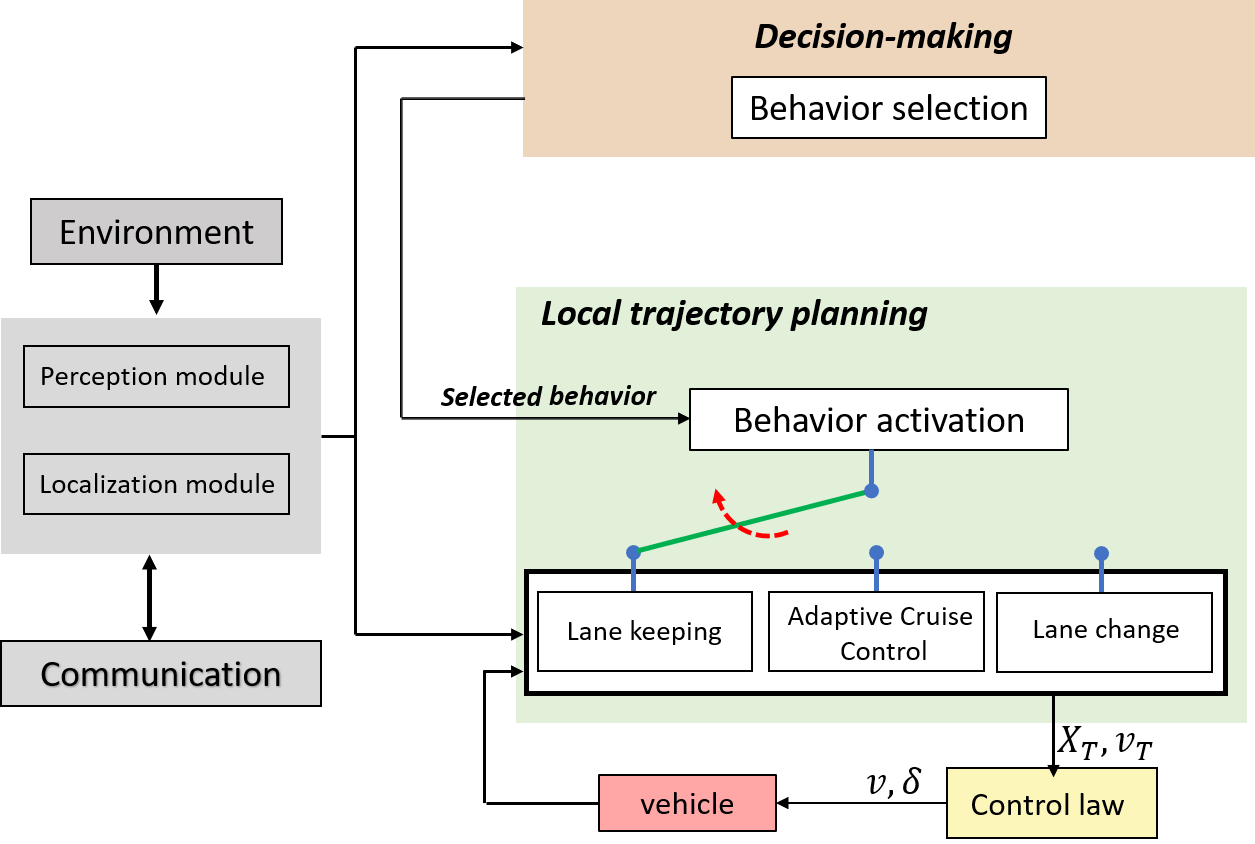
\includegraphics[width=11cm,height=18cm,keepaspectratio]{chapters/Chapitre_4/Figures/Adapted_control_architecture.png}
       % \vspace{-2.3mm}
        \caption{Multi-Controller Architecture}
        \label{fig:MCA}
       % \vspace{-5mm}
        \end{figure}







Building upon the MCA paradigm outlined in this section, the subsequent section provides an overview of the main functionalities of the proposed C-MCA tailored for merging onto highway on-ramps in the context of MVS. Special attention is given to the decision-making and planning levels.




% Cooperative Navigation (CN) stands as a widely adopted approach to ensure the effective maneuvering of intelligent vehicles within complex/cluttered environments. As discussed in Section \ref{sec: CooperativeNavigation-Scenarios Overview}, the coordination complexities arising in both rural and urban settings encompass tasks such as harmonizing speeds on motorways and highways, facilitating smooth merging on on-ramps, and orchestrating the movements of the vehicles on highways. However, the primary hurdle lies in accurately assessing and mitigating potential hazards within the road environment while implementation adaptable CN strategies, as discussed in Section \ref{sec: CooperativeNavigation_GlobalOverview}. Consequently, the main aim of this Ph.D. thesis is to propose a safe and energy efficient control architectures for MVS that navigates in dynamic and complex environment such as merging on on-ramp and multi-road navigation on highway,  with a reasonable communication conditions. 

% % il faut parler du contenue de ce chapitre en précisant les items qui y figurent 
% More precisely, this chapter firstly outlines in Section \ref{sec: problem_statement} the the general problem statement tackled in this PhD along with the main related challenges. The global decision/control architecture proposed in the context of this PhD is given in Section \ref{sec: AFRS}. 



















\section{Overall Cooperative Multi-Controller Architecture} \label{sec: AFRS}

% pour l'architecture proposée on peut citer les items suivants: 
% - commencer par la partie architecture global avec les modules mais d'un point de vu global 
% - dire que les modules perceptions et localization sont déjà traités avant dans les sections et les citer 
% - mettre l'ascent sur les architectures multi-controller et les systèmes de selection de comportement (switch, etc) 
% - introduire notre propre architecture, et expliquer les modules et leurs fonctionnement ! 


\subsection{The C-MCA main functionalities}






The primary focus of this work revolves around adapting the MCA detailed in Section \ref{sec:MCA}, to suit the requirements of cooperative navigation within the MVS paradigm in complex and dynamic environments. More precisely, it is proposed to employ the MCA as the foundational framework in the development of a Cooperative Multi-Controller Architecture (C-MCA) (cf. Figure \ref{fig:C-MCA}) designed to overcome the challenges related to MVS navigation on on-ramp merging and cooperative highway navigation. 

The proposed C-MCA is depicted in Figure \ref{fig:C-MCA}. It has been designed around various interconnected modules that facilitate planning, control, access, and management of on-ramp merging and cooperative highway navigation within MVS. This section aims to establish a global focus of the main functionalities part of the C-MCA, whith an emphasis on the decision-making level (cf. Figure \ref{fig:C-MCA} \textcircled{\small{1}}) and the local trajectory planning (cf. Figure \ref{fig:C-MCA} \textcircled{\small{2}}).  























\subsubsection{Environment perception} \label{sec:environment_features}
As discussed in both Section \ref{sec: perception} and Section \ref{sec: localization}, the roles of the perception and localization modules involves furnishing the essential environmental characteristics indispensable for MVS navigation. These characteristics encompass critical information such as the vehicle's precise localization, the number of lanes, lane markings, distances to road boundaries, and the pose of detected obstacles. To achieve this, these modules operate based on a vector map, serving as a detailed representation of the environment. Fusion algorithms, combining data from perception and localization, are employed to generate a reliable representation of the environment. 


\textbf{\textit{Assumption 1:}} It is essential to underscore that this PhD manuscript concentrates on the decision-making and planning/control modules with the C-MCA. Consequently, the perception, localization, and vector map modules are assumed to be reliable and are not the primary focus of this research.  





\newpage
\thispagestyle{empty}
\begin{landscape}
        \begin{figure}[!h]
        \centering 
        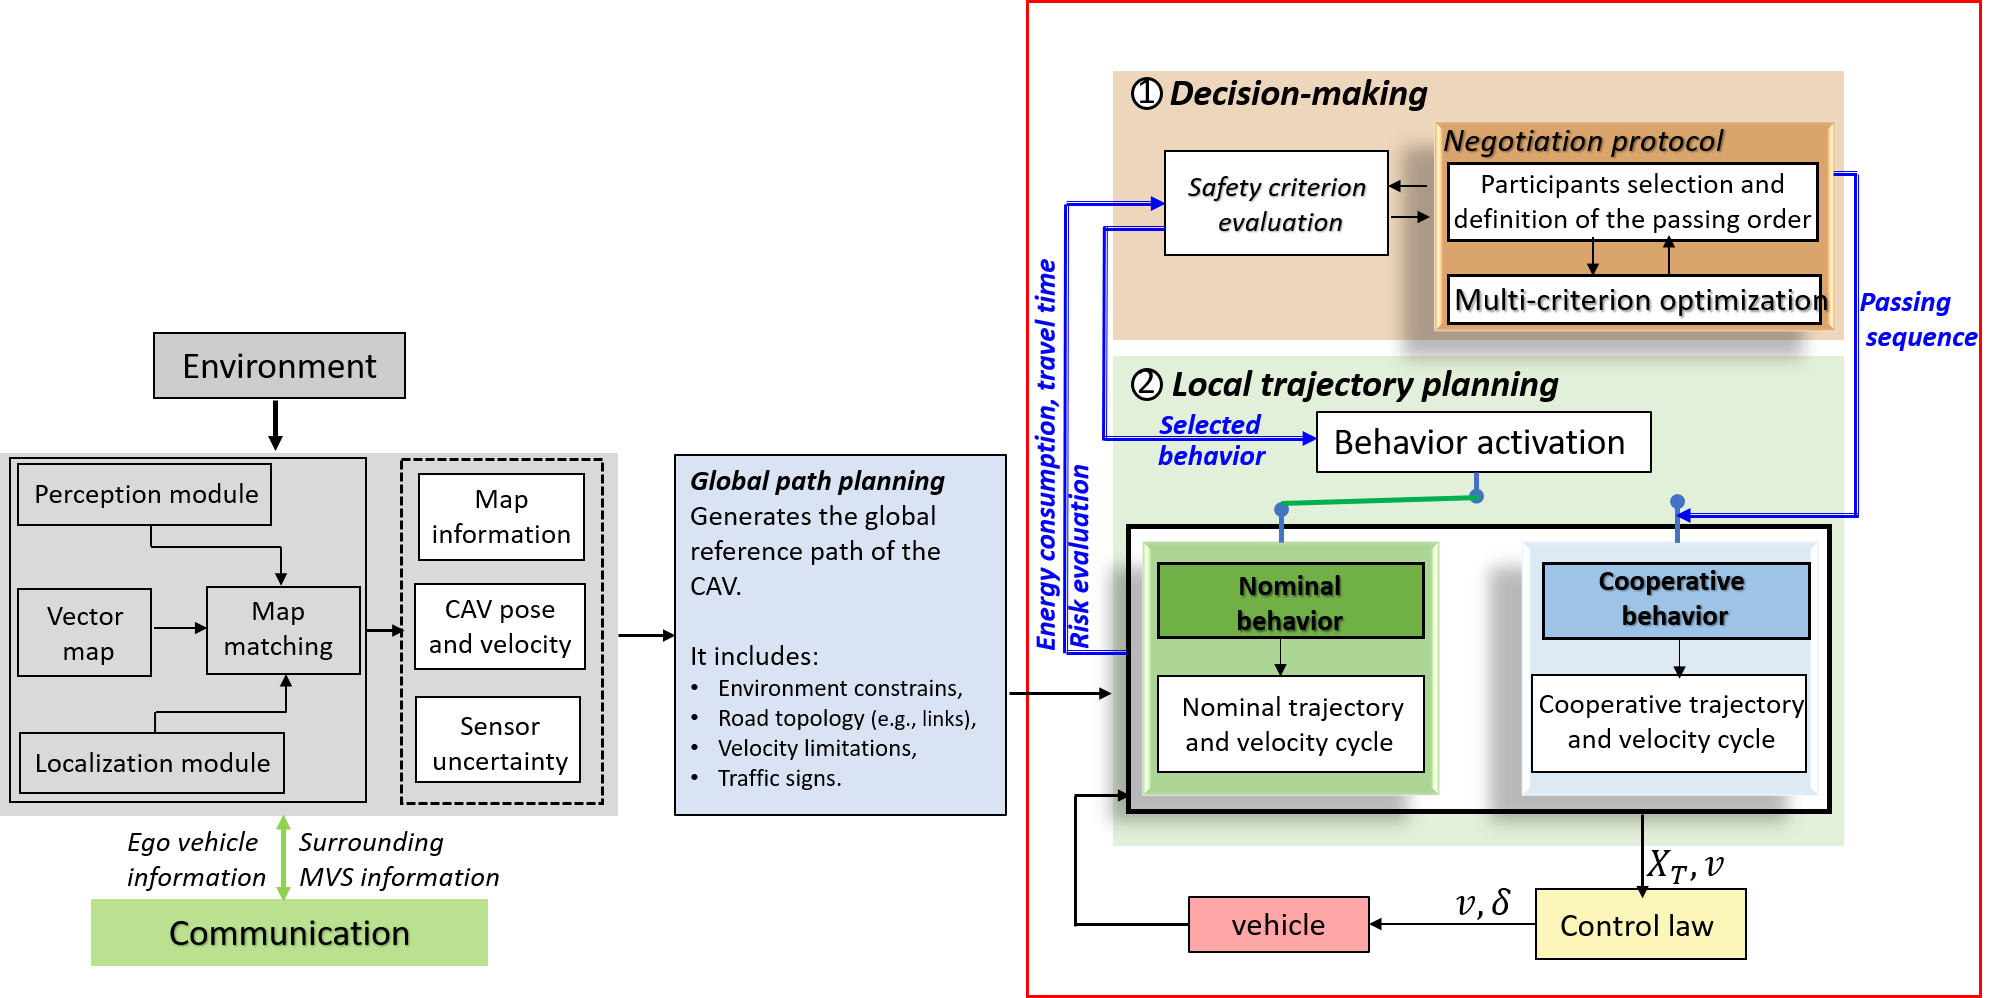
\includegraphics[width=20cm,height=18cm,keepaspectratio]{chapters/Chapitre_4/Figures/C_MCA.png}
        \vspace{-2.3mm}
        \caption{Cooperative Multi-Controller Architecture }
        \label{fig:C-MCA}
        \vspace{-5mm}
        \end{figure}


\end{landscape}
















\subsubsection{Communication module} \label{sec:communication_module}
  This module operates in collaboration with the Road Side Unit (RSU) positioned within the merging zone (cf. Figure \ref{fig:ScenarioTopology}). The RSU acts as a conduit for the exchange of crucial information between the merging vehicle and the highway vehicles, thus enhancing of the MVS's motion coordination capabilities. In essence, when referring to the communication aspect of this research, it pertains to the exchange of information between the vehicle components of the MVS and the RSU, all within the communication range defined in Figure \ref{fig:ScenarioTopology}. Further details related to the RSU can be found in Appendix \hyperlink{AppendixA}{A}). 

\textbf{\textit{Assumption 2:}} It is important to note that the communication module, both within the vehicles and integrated into the RSU, functions as tools aimed at enhancing the overall abilities of the MVS.  However, it is crucial to acknowledge that the complexities inherent in the levels addressed in this research preclude the comprehensive investigation of communication-related aspects such as communication delays, packet losses, and dynamic communication topologies. 
















\subsubsection{Global path planning}\label{sec:global_planner} 
The global path planner module gives a selected sequence of way-points through the road network. Additionally, it has the responsibility of setting the goal of the vehicle (e.g., its destination, navigating lane, etc.). It uses the inputs of the perception modules to cope with the traffic road rules 
(e.g., speed limits, traffic signs, etc.).










% \subsubsection{Risk assessment and management module} \label{sec:risk_assessment} 
% The principal objective of the risk assessment and management module is to uphold the paramount safety criterion consistently. This module has been devised to interpret the environment feature data and determine whether the decision-making level possesses the capacity to ensure compliance with safety criterion. In cases where such assurance is lacking, this module can trigger a fail-safe procedure. 








\subsubsection{Decision-making level} \label{sec:decision_making}
After defining the environmental perception and the vehicle's global path, it becomes imperative to adopt an appropriate decision-making strategy for the vehicle component within the C-MCA. This strategy must consider various factors, including the vehicle's objectives, the MVS overarching objectives, traffic regulations, etc. 



The core requirement of the decision-making level is to ensure the safety of the MVS during the on-ramp merging maneuver. Consequently, given the shared nature of on-ramp merging scenario and the high dynamic relative to the highway, the decision-making must establish a strategy to solve the conflicting scenarios. Before delving into the presentation of the proposed decision-making level part of the C-MCA, a short overview of the literature approaches used to solve the conflicts part of the shared zones is proposed.



As with intersection crossing, the merging conflict is mainly justified because of the shared nature of the merging zone \cite{mariani2021coordination}. Thus, solving conflicting scenarios requires an appropriate strategy designed to take into account explicitly these conflicting configurations. Several strategy can be found in the literature and they can be mainly classified in two categories:  (1) Centralized approaches and Decentralized approaches. In Centralized approaches, a Central controller defines the passing sequence of the vehicle in the shared zone, and the vehicles have no words concerning the selection policy. In contrast, in decentralized approaches, negotiation-based strategy can be used to establish the passing sequence. Some contributions part of the intersection crossing and on-ramp merging literature focused on the competitive nature of the  scenario \cite{mariani2021coordination}. Thus, the use of negotiation can be performed with auction-based mechanism. While approaching the shared zone, each vehicle can contact the RSU and place a bid; place an offer to buy a portion of the shared zone for a certain period. The value of the bid expresses the urgency of the vehicle. The RSU collects the bids and accord the conflict portion to the vehicle that placed the highest bid \cite{carlino2013auction}\cite{cabri2019auction}\cite{vasirani2012market}. The main limitation of the auction-based strategy is the liveness of the method, i.e., as explained in  \cite{mariani2021coordination} liveness stands for starvation of the vehicles; in some cases, the constant bidding strategy of the vehicle can prevent other vehicles from wining an auction, with the risk for them an indefinitely waiting time. 



        \begin{figure}[!h]
        \centering 
        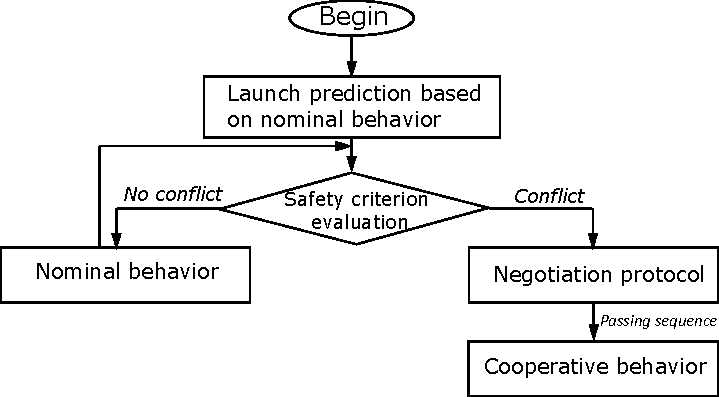
\includegraphics[width=12cm,height=18cm,keepaspectratio]{chapters/Chapitre_4/Figures/Decision-making-level.pdf}
       % \vspace{-2.3mm}
        \caption{Flowchart of the decision-making level part of the C-MCA}
        \label{fig:Decision-module}
        %\vspace{-5mm}
        \end{figure}



In this PhD work, instead of relying on the competitive nature of the on-ramp merging scenario, it is proposed to rely on its cooperative nature. Consequently, the conflicting is solved while ensuring the respect of the MVS overarching goal and vehicle's individual goals. The decision-making level within the C-MCA module is founded upon a multi-behaviors decision-making system. This decision-making module (cf. Figure \ref{fig:C-MCA} \textcircled{1}) is responsible for selecting one of the two operational behaviors within the local trajectory level (cf. Figure \ref{fig:C-MCA} \textcircled{2} and Figure \ref{fig:Decision-module}), with respect to the safety criterion. In simpler terms, the decision-making level prompts the nominal behavior (responsible for promoting the vehicle's individual goals) to make predictions about the vehicle's expected nominal motion (cf. Figure \ref{fig:Decision-module} and Figure \ref{fig:C-MCA} \textcircled{2}). Based on these predictions, the safety criterion is assessed, if the nominal behavior is safe then the latter is activated. However, when a conflicting merging is detected based on the nominal behavior, the decision-making level and the cooperative behavior works together to solve the conflict (cf. Figure \ref{fig:Decision-module} and Figure \ref{fig:C-MCA} \textcircled{1} \textcircled{2}), while respecting both the MVS overarching goal and the vehicle's  individual goals. Further details about the multi-behavior decision-making level part of the C-MCA can be found in Chapter \ref{Chap05}. 





















\subsubsection{The local trajectory planning level} \label{sec:local_planning}
The local trajectory planning level part of the C-MCA in Figure \ref{fig:C-MCA} is composed of two primary behaviors: 

\begin{enumerate}
\item The nominal behavior: It takes into account data from the environment perception, and global path planning modules to predict the expected behavior of each vehicle within the MVS. The nominal behavior is designed to achieve the MVS vehicle's individual goals, thus it is optimized to enhance the performance of the involved vehicle. The forecaster behavior is subsequently evaluated using a safety metric by the decision level within the C-MCA, further details can be found in Section \ref{sec:The_nominal_mode}. 

\item The cooperative behavior: In cases where the nominal behavior fails to adhere to the safety criterion, the C-MCA decision-making level activates the cooperative behavior. Consequently, the cooperative behavior receives additional inputs, including safety evaluations related to the nominal behavior, in addition to the selected passing sequence. Based on these inputs, the cooperative behavior has the responsibility of generating the vehicles' dynamics corresponding to the passing sequence. The translation of the passing sequence into the MVS dynamics is ensured by the formation control strategy part of C-MCA.  Further details about the formation control strategy are given in Chapter \ref{Chap04}. 




\end{enumerate}






\subsubsection{The control level} \label{sec:control_law}
The control level is tasked with the precise tracking of the set-points generated by the local planning level. These set-points serve as a reference for the control to follow. The local trajectory planning level creates a velocity profile and yaw rate that are well-suited for the vehicle.

The used control law is the one detailed in Section \ref{sec:control_law}. The control law is synthesized for a tricycle model-based vehicle (cf. Section \ref{sec:control_law}) using Lyapunov  synthesis and is detailed in Section \ref{sec:control_law}. 



% je ne sais pas s'il faut ajouter une phrase de transition ici ou pas ... 


\section{Problem statement} \label{sec: problem_statement}
% ajouter une partie ou on parle du scenario qu'on cherche à traiter dans cette thèse avec toute la topologie de la route etc. Un peu comme le fait déjà zhang enfaite :! -- voir mon carnet de notes 
% il faut aussi présenter les hypothèses de travail qu'on fait tout au long de cette thèse comme celle sur la communication par example ! 
% il faut aussi expliquer comment la communication intervient dans l'architecture et comment les tâches sont distribuées entre les différents véhicules etc 





As previously discussed in both Chapter \ref{chap:chapter2} and Chapter \ref{Chap03}, and as highlighted by the comprehensive literature reviews in  \cite{bernardin2019scenario} \cite{guo2019urban} \cite{wang2019survey} \cite{7562449}, the coordination challenges confronting MVS extend their influence over a wide array of environments, encompassing both rural and urban settings, including highways. These challenges manifest in a multitude of scenarios, including the imperative for coordination on highways to maintain uniform speeds, as well as the intricacies of merging onto and exiting from on-ramps. As elucidated in Section \ref{sec: CooperativeNavigation-Scenarios Overview}, the cooperative navigation of MVS on highways ushers in an array of driving benefits, ranging from enhancing safety to improved traffic flow and optimized energy efficiency (cf. Section \ref{sec: CooperativeNavigation-Scenarios Overview}). 


In this section, we aim to provide an overview of the background that underlies this PhD thesis. Section \ref{sec:ScenarioTopology} will present a representation of the highway scenario involving on-ramp, thereby establishing the overarching road topology that serves as the foundational scenario of this work. Subsequently, the control law used in this PhD work is detailed. Lastly, the formalism definition and modeling of the formation are discussed. 


\subsection{Scenario topology}\label{sec:ScenarioTopology}

This research endeavors to leverage the capabilities of MVS to confront the intricacies associated with cooperative highway navigation. More precisely, it sets out to address the challenging scenario of cooperative merging at highway on-ramps, a scenario associated with significant safety and mobility complexities. The specific use at the heart of this research is illustrated in Figure \ref{fig:ScenarioTopology}, encompassing a multi-lane highway environment incorporating an on-ramp as the entry point to the highway section. Additionally, this scenario accounts for a designated merging zone, characterized by a fixed length, where merging maneuvers are authorized. Furthermore, the prescribed speed limits governing both the highway and the on-ramp segments are integrated as predetermined parameters with this scenario. 



        \begin{figure}[!h]
        \centering 
        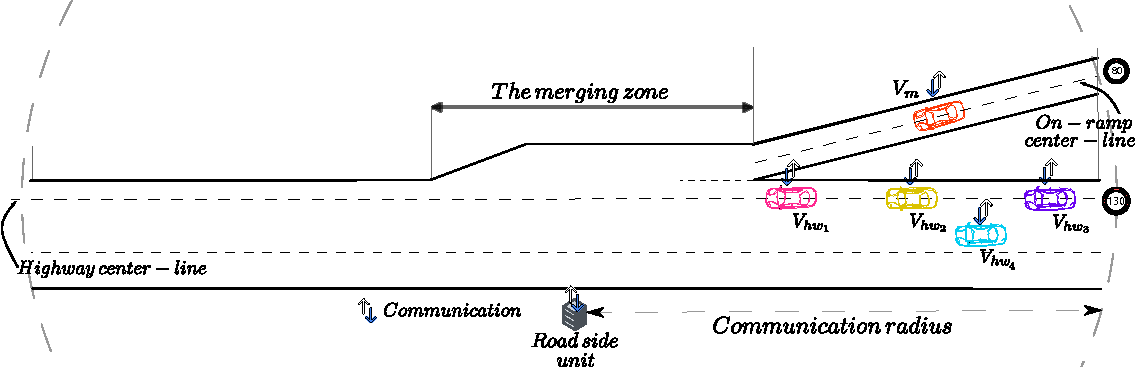
\includegraphics[width=12.5cm,height=18cm,keepaspectratio]{chapters/Chapitre_4/Figures/ScenarioScene.pdf}
        \vspace{-2.3mm}
        \caption{Illustration of the scenario topology of the on-ramp merging on highway}
        \label{fig:ScenarioTopology}\label{fig:RSU-identification}
       % \vspace{-5mm}
        \end{figure}




The distinctive feature of the on-ramp merging scenario is the complex motion synchronization hurdles encountered by the vehicles. These challenges materialized as vehicles on the on-ramp must make decisions about whether to accelerate or decelerate. All this, while ensuring a safe and continuous merge onto the desired highway lane, often under conditions where a clear line of sight is not guaranteed. Simultaneously, highway users must adapt their speeds to accommodate to the behavior of the merging vehicle, which can potentially disrupt the flow of traffic and result in congestion. One way to help synchronization ability of the vehicles participating in the merging scenario is with the help of communication. In this work, we take the assumption of a on-ramp merging scenario equipped with a Road RSU (cf. Appendix \hyperlink{AppendixA}{A}).  


\subsection{Control law } \label{sec:control_law}

Before presenting the used control law, it is important to know the vehicle's model. 



Assuming that the vehicle evolves in asphalt road and in cluttered urban environment with relatively low speed, the following model is based on tricycle model \cite{ventura2015safe}. The two front wheels are replaced by a single virtual wheel located at the center of both front wheels. 


\begin{equation} \label{eq:vehiclemodel}
\begin{aligned}
\dot{x} &=v \cos (\theta) \\
\dot{y} &=v \sin (\theta) \\
\dot{\theta} &=v \tan (\gamma) / l_{b}
\end{aligned}
\end{equation}

\noindent $(x,y,\theta)$ is the vehicle's pose on the global reference frame $X_{G},Y_{G}$. $v$ is the vehicle's linear velocity and $\gamma$ is the steering angle of the vehicle. $l_{b}$ is the vehicle's wheelbase. $v$ and $\gamma$ are the control inputs of the vehicle (cf. eq \ref{eq:vehiclemodel}). 



	\begin{figure}[!h]
	\begin{center}
		
		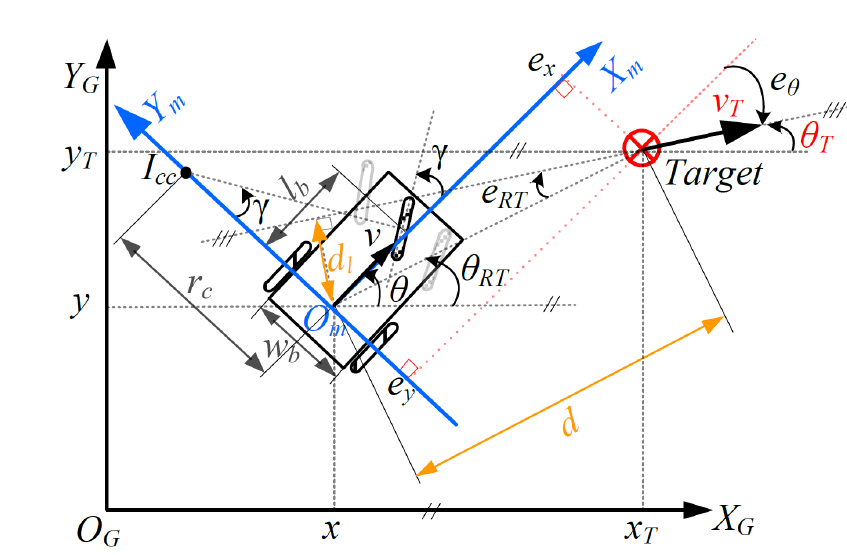
\includegraphics[width=120mm,height=80mm]{chapters/Chapitre_4/Figures/vehicle_tricycle model.PNG}\\
		\caption{	\label{fig:vehicle_tricycle_model}Vehicle’s and target’s configuration in global $(X_G; Y_G)$ and local $(X_m; Y_m)$ reference
frames, and the control variables \cite{ventura2015safe}}
		
		
		
	\end{center}
\end{figure}



According to Figure \ref{fig:vehicle_tricycle_model}, $w_b$ corresponds to the track width of the vehicle and $I_{cc}$ the instantaneous center of curvature of the vehicle trajectory. The radius of curvature $r_c$ is given by: 

\begin{equation}
    r_c=\frac{l_b}{tan(\gamma)}
\end{equation}

\noindent and $cc=1/r_c$ is the curvature of the vehicle trajectory. \\




The used control law \cite{vilca2015novel} aims to drive the vehicle toward specific targets (static or dynamic) in the environment. At each sample time the tracked target is defined by a posture $(x_T,y_T,\theta_T$) and velocity ${V}_T$ (this velocity could be equal to 0 if the target is static). Using a Lyapunov formulation, the used control law \cite{vilca2015novel} is presented below. 

The adopted Lyapunov function $V$ is given by eq. \ref{eq:lay_control_1}. 

\begin{equation}\label{eq:lay_control_1}
\begin{aligned}
V & =\frac{1}{2} K_d d^2+\frac{1}{2} K_l d_l^2+K_o\left[1-\cos \left(e_\theta\right)\right] \\
& =\frac{1}{2} K_d d^2+\frac{1}{2} K_l d^2 \sin ^2\left(e_{R T}\right)+K_o\left[1-\cos \left(e_\theta\right)\right]
\end{aligned}
\end{equation}


\noindent where the initial values of $e_{R T}$ and $e_\theta$ must satisfy the following initial conditions:
\begin{equation}
    e_{R T} \in ]-\pi / 2, \pi / 2\left[\text { and } e_\theta \in \right]-\pi / 2, \pi / 2[
\end{equation}

The Lyapunov function (cf. eq. \ref{eq:lay_control_1}) is therefore a function of three parameters which depend on: the distance $d$ between the target and vehicle's position; the distance $d_l$ from the vehicle to the target line (line that passes through the target position with an orientation equal to the target orientation), this term is related to the Line of Sight and Flight of the target; and the orientation error $e_\theta$ between the vehicle and the target.


The desired linear velocity $v$ and the front wheel steering $\gamma$ of the vehicle which allow to asymptotically stabilize the error vector $\left(e_x, e_y, e_\theta,\left(v-v_T\right)\right)$ toward zero (permitting therefore to have $\dot{V}<0$) are given by:

\begin{equation}
\begin{aligned}
v & =v_T \cos \left(e_\theta\right)+v_b \\
\gamma & =\arctan \left(l_b c_c\right)
\end{aligned}
\end{equation}

\noindent where $v_b$ and $c_c$ are defined by: 
\begin{equation}
v_b=K_x\left[K_d e_x+K_l d \sin \left(e_{R T}\right) \sin \left(e_\theta\right)+K_o \sin \left(e_\theta\right) c_c\right]
\end{equation}
with: 
\begin{equation}
\begin{aligned}
c_c= & \frac{1}{r_{c_T} \cos \left(e_\theta\right)}+\frac{d^2 K_l \sin \left(e_{R T}\right) \cos \left(e_{R T}\right)}{r_{c_T} K_o \sin \left(e_\theta\right) \cos \left(e_\theta\right)}+K_\theta \tan \left(e_\theta\right) \\
& +\frac{K_d e_y-K_l d \sin \left(e_{R T}\right) \cos \left(e_\theta\right)}{K_o \cos \left(e_\theta\right)}+\frac{K_{R T} \sin ^2\left(e_{R T}\right)}{\sin \left(e_\theta\right) \cos \left(e_\theta\right)}
\end{aligned}
\end{equation}

\noindent $K=(K_d, K_l, K_o, K_x, K_\theta, K_{RT})$ is a vector of positive constants defined by the designer. Accurate analysis of this stable and efficient control law is given in \cite{vilca2015novel}\cite{ventura2015safe}. 

\subsection{Formation definition and configuration}\label{sec:formation_modeling_section}







Based on the MVS paradigm (cf. Section \ref{sec:MVS-paradigm}) and the communication range of the RSU (cf. Figure \ref{fig:ScenarioTopology}), a set of $N$ vehicles involved in creating the formation is identified. In other words, the RSU establishes connections with all the vehicles within its communication range. Consequently, the RSU assigns a unique communication identifier, in addition to the definition of the reference vehicle used as a reference frame by the formation coordinate system. This strategy is defined as follows: 

\begin{itemize}
    \item \textbf{Reference vehicle:} The RSU has the responsibility of designating the reference vehicle $V_R$ (cf. Figure \ref{fig:RSU-identification}). The pose of the latter is used as a mobile reference frame by the formation coordinates system. The RSU can select $V_R$ either from the vehicles part of the MVS or by considering a virtual vehicle. In this thesis work, the reference vehicle $V_R$ is selected from the MVS vehicles traveling in the lane containing the merging zone, and based on the shortest distance w.r.t. merging zone (cf. Figure \ref{fig:RSU-identification}). Its position is denoted by $x_{\text{R}}, y_{\text{R}}$, and its velocity by $\mathcal{V}_{\text{R}}$.
    
    
 

    \item \textbf{Formation modeling approach:} The formation of MVS is structured based on the virtual structure approach (cf. Section \ref{sec: Virtual-structure}). Figure \ref{fig:Coordinates_system} presents the formation coordinates  $F={f_i,i=1,\ldots,N}$, where $f_i$ are the $i-th$ vehicle coordinates w.r.t. the reference frame of the formation. 

    
% \end{itemize}
%        \begin{figure}[!h]
%         \centering 
%         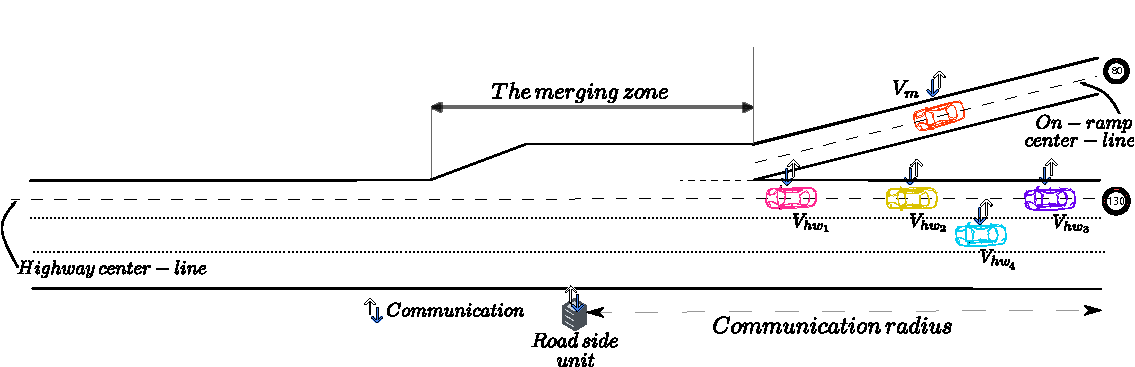
\includegraphics[width=14cm,height=6cm]{chapters/Chapitre_5/Figures/RSU_identification.pdf}
%         %\vspace{-2.3mm}
%         \caption{Formation identification and id attribution}
%         \label{fig:RSU-identification}
%         %\vspace{-5mm}
%         \end{figure}





\subsubsection{Formation modeling based on a dynamic reference frame}


In Figure \ref{fig:RSU-identification}, the RSU broadcast $V_{R}$ pose to the vehicles part of the formation in order to compute their coordinates w.r.t. $V_R$ reference frame. According to \cite{8430659}, two suitable frames for formation definition can be used: 


\begin{itemize}
    \item \textbf{Cartesian reference frame:} also called rigid formation, it aims to maintain the formation's shape, the positions and orientations of the vehicles within the formation, computed relative to $V_{R}$, which is also called the leader vehicle, with respect to the Cartesian reference frame (the local frame of the reference vehicle defined as $X_m$ and $Y_m$). This approach aims to reduce vehicle's dependence on a global reference frame. Applying a straightforward transformation allows the determination of the vehicles part of the formation coordinates within a local reference frame attached to the reference vehicle \cite{mariottini2007leader}\cite{benzerrouk2010navigation}.

    \item \textbf{Frenet reference frame:} \label{sec:FrenetFrame} also known as flexible formation, this approach is utilized when it is more critical to track the reference vehicle's movements than to maintain a fixed formation shape during navigation. The Frenet reference frame is employed to adapt the formation to the reference vehicle's trajectory. This trajectory is used to define the formation's longitudinal (curvilinear) and lateral (perpendicular to the trajectory) coordinates \cite{8430659}\cite{avanzini2010urban}\cite{klanvcar2011control} (cf. Figure \ref{fig:Coordinates_system}).
\end{itemize}








In the Cartesian formation, the reference vehicle path is not taken into account such as in the Frenet formation, only its current Cartesian pose and dynamics have to be known by the vehicles part of the formation. Since the reference vehicle trajectory is part of the Frenet formation modeling, the latter offers a safe formation navigation in static environment. In contrary, according to \cite{8430659}, the Cartesian formation allows a safe stable geometric formation shape. 

During the on-ramp merging scenario, the formation shape is reconfigured from one initial shape to another, while guaranteeing the safety of the reconfiguration. Based on the advantages of both of the formation modeling approaches, the Frenet modeling approach is the one that satisfies the scenario requirements. In fact, one of the particularities of the on-road environment is its high dynamic, especially for highway environment. Additionally, the Frenet modeling approach offers more flexibility, an important requirement for navigation in dynamic environments. 

\subsubsection{Formation modeling based on the Frenet reference frame}
Each vehicle part of the formation is characterized by its coordinates $X_i=[x_i,y_i]^T$ within the global reference frame $[X_G,Y_G]$ (cf. Figure \ref{fig:Coordinates_system}). In order to locate $X_i$ w.r.t. the reference vehicle $V_R$ (cf. Figure \ref{fig:Coordinates_system}), it is proposed to use a Frenet reference frame (cf. Section \ref{sec:FrenetFrame}) centered on $V_R$ (cf. Figure \ref{fig:Coordinates_system}). 

       \begin{figure}[!h]
        \centering 
        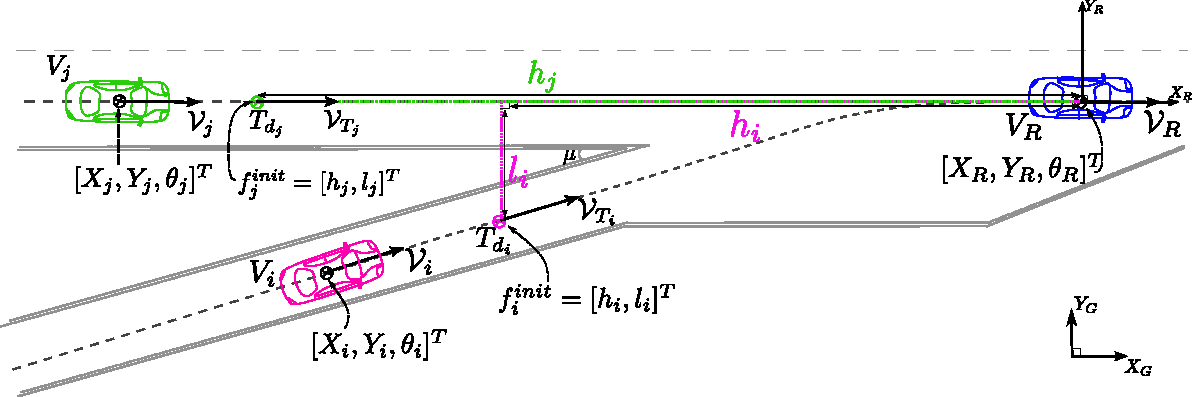
\includegraphics[width=12.5cm,height=18cm,keepaspectratio]{chapters/Chapitre_5/Figures/ModelingScenarioSimple.pdf}
        %\vspace{-2.3mm}
        \caption{Coordinates system based on the Frenet reference frame}
        \label{fig:Coordinates_system}
        %\vspace{-5mm}
        \end{figure}



According to $V_R$ pose $X_R$ and its reference trajectory (cf. Figure \ref{fig:Coordinates_system}), the coordinates system is described as follows: 

\begin{itemize}
    \item The $i-$vehicle coordinates part of the formation are defined as $f_i=[h_i,l_i]^T, i\in {N}$ (cf. Figure \ref{fig:Coordinates_system}). 

    \item $h_i$ and $l_i$ are the longitudinal and lateral vehicle's coordinates w.r.t. the Frenet reference frame, respectively. The longitudinal coordinate $h_i$ represents the curvilinear distance between $V_R$ and $X_i$ according to the tangent to $V_R$ trajectory, while the lateral coordinate $l_i$ is computed based on the perpendicular line between $X_R(h_i)$ and its reference trajectory, and that passes through $X_i$, $l_i=PerpDist{X_R(h_i),X_i}$ (cf. Figure \ref{fig:Coordinates_system}). 
\end{itemize}


The kinematic model in eq. \ref{eq:vehiclemodel} is written in the global reference frame ${X_G, Y_G}$, thus a transformation from the mobile reference frame to the global reference frame is obtained with the following equations: 

\begin{equation} \label{eq:frenetToCartisian}
\begin{matrix}
\begin{bmatrix}
x_{T_i} \\
y_{T_i} \\
\end{bmatrix}
& = & \begin{bmatrix}
x_{R}(h_i)\\
y_{R}(h_i) \\
\end{bmatrix}
& + & \begin{bmatrix}
-l_i\sin(\theta_R(h_i)) \\
l_i\cos(\theta_R(h_i)) \\
\end{bmatrix}
\end{matrix}
\end{equation}


with $[x_{T_i},y_{T_i}]^T$ is the i-th vehicle virtual target w.r.t. $V_R$'s mobile reference frame. $[x_R,y_R]^T$ and $\theta_R$ are the reference vehicle $V_R$ pose and orientation.



       % \begin{figure}[!h]
       %  \centering 
       %  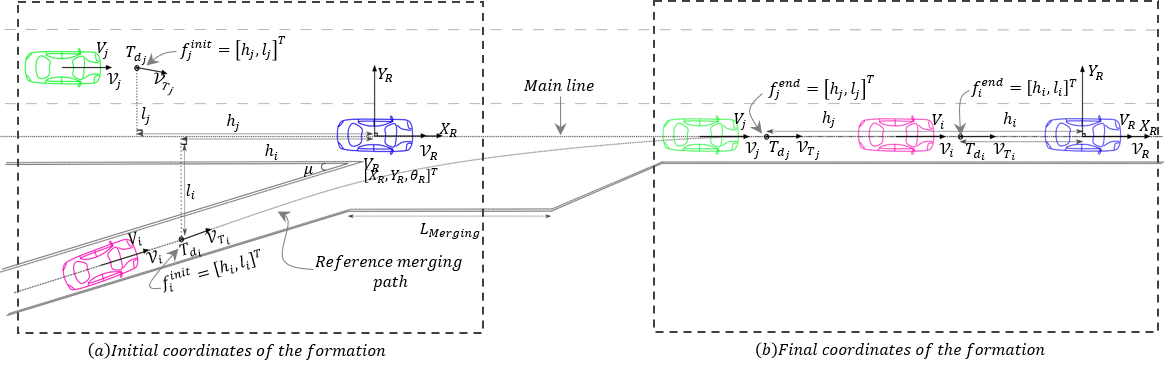
\includegraphics[width=14cm,height=6cm]{chapters/Chapitre_5/Figures/Full_scenario.png}
       %  %\vspace{-2.3mm}
       %  \caption{The virtual structure approach used to model the formation and its reconfiguration to perform the merging maneuver. (a) The initial shape of the formation and its coordinates. (b) The final shape of the formation after the merging maneuver and its desired coordinates. }
       %  \label{fig:Coordinates_system_full_scenario}
       %  %\vspace{-5mm}
       %  \end{figure}











\section{Conclusion}

This chapter presented the design of the Cooperative Multi-Controller Architecture (C-MCA) for safe and energy efficient on-ramp merging on highway, in addition to the details given on the main modules, as well as, their interactions. Indeed, the C-MCA aims to satisfy both the MVS overarching goal and the vehicle's individual goals. With the help of the multi-behavior decision-making level part of the architecture, the nominal behavior is activated when it is safe to satisfy the vehicle's individual goals. Satisfying the vehicle's goals is not always possible, especially given the shared nature of the merging zone. Consequently, the C-MCA has a dedicated cooperative behavior that works along the negotiation protocol part of the decision-making level to solve conflicting merging scenarios. In fact, a safe passing sequence is selected by the decision-making level, and the latter is translated into the vehicle's dynamics by the formation control approach part of the cooperative behavior. The following chapter is dedicated to present the details related to the proposed formation control strategies. 